\section{Architektur}
Für die Realisierung der GDPR konformen Datenverarbeitung ohne die Erteilung eines Verarbeitungsauftrages an das jeweilige \ac{CSP} soll Intel SGX eingesetzt werden. Intel SGX bietet die Möglichkeit gesicherte Programmbereiche auszuführen, sodass von extern kein Zugriff möglich ist. Diese Funktionsweise bildet die geschützte Datenverarbeitung innerhalb eines Rechenzentrums ab, ohne eine Zugriffsmöglichkeit direkt von anderen Instanzen auf der physikalischen Maschine sowie den indirekten Zugriff über die Infrastruktur durch das \ac{CSP}. 

In \autoref{img:sgx-idea} ist der Aufbau skizziert. Der grüne Bereich repräsentiert hierbei den vertrauenswürdigen Bereich und die direkte Zuständigkeit eines beliebigen Unternehmens. Auf der rechten Seite ist dieses Unternehm abgebildet, welches über verschiedene Clients verfügt und über eine gesicherte Verbindung auf den Datencontainer bei einen Hosting Container zugreifen möchte. 

\begin{figure}[h!]
	\centering
	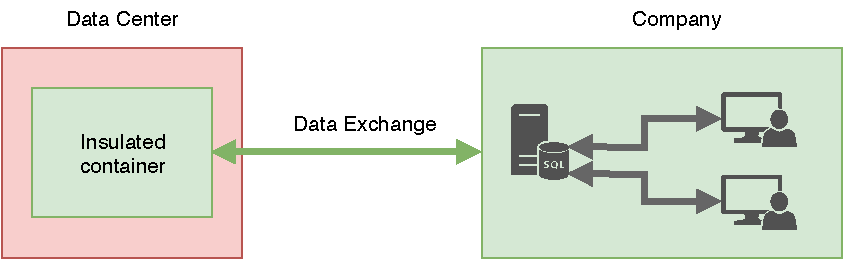
\includegraphics{img/sgx_idea/sgx-idea.pdf}
	\caption{Skizzierung des Ziels einer gesicherten Umgebung bei einem \ac{CSP}}
	\label{img:sgx-idea}
\end{figure}

\subsection{Intel SGX}
 In diesem Abschnitt werden lediglich die wichtigsten Komponenten beschrieben, welche für das Verständnis der Architektur notwendig sind. Intel SGX ermöglicht die Bereitstellung von sicheren Programmumgebungen, die sogenannten \emph{Enclaves}. Eine Enclave besteht aus zwei essentiellen Bestandteilen. Das Rahmenwerk einer Enclave definiert der \emph{Unsecure Part},  welcher keinerlei Schutzfunktionen unterliegt, jedoch die Schnittstellen zu dem eigentlichen, gesicherten Container innerhalb einer Enclave beinhaltet.
 
 Die Enclaven werden innerhalb dem \ac{DRAM} abgelegt. In diesem existiert ein zusammenhängender Speicherbeich, welche den sogenannten \ac{PRM} beinhaltet. Auf diesen Bereich kann durch die Software nicht direkt zugegriffen werden. Der \ac{PRM} beinhaltet wiederum einen Speicherbereich, welcher \ac{EPC} bezeichnet wird. Der \ac{EPC} enthält alle Enclaves, die auf dem jeweiligen System agieren \cite{sgx-bibel}. Hierbei ist zu erwähnen, dass die parallele Ausführung mehrere Enclaves möglich ist.
 
 Die maximale Größe des \acs{EPC} beträgt 128 MiB. Hiervon können 93 MiB aktiv genutzt werden. Übersteigt eine Enclave die genannte Größe, so ist das kostspielige Swapping über den \ac{EPC} notwendig. \cite{sgx-performance} Programme, die innerhalb einer Enclave ausgeführt werden können, sind in den Programmiersprachen \emph{C} oder \emph{C++} zu schreiben. Zudem ist es grundsätzlich möglich beliebige Programmbibliotheken der jeweiligen Programmiersprache zu importieren.
 
 \subsection{Struktur einer Enclave}
 In diesem Abschnitt die die Struktur der Enclave betrachtet werden, welche genutzt wird, um Anfragen zu bearbeiten. Der erwähnte Use-Case ist das Handling von Datenbankoperationen auf einer verschlüsselten \ac{SQL} Datenbank. Das Interface für die gesicherte, externe Kommunikation wird zunächst abstrahiert. Es wird davon ausgegangen, dass die \ac{SQL} Instruktionen über ein sicheres Verfahren die Enclave erreichen. Diese stellt hierfür ein External Interface bereit. Diese Interface wird innerhalb des \emph{Unsicheren Bereichs} ausgeführt. Die Datenkommunikation dient hierbei lediglich als Relay und wird an das \emph{Communication Interface} des sicheren Bereichs weitergeleitet. \\
 
 
 Anschließend wird mit der $EncryptionEngine_{External}$ die Anfrage entschlüsselt und die extrahierten Instruktionen an den \emph{SQL Handler} weitergereicht. Parallel wird eine Anfrage an die $EncryptionEngine_{Storage}$ gestellt, welche die erforderlichen Daten anfragt. Auf Grund der möglichen Dimensionen einer Datenbank, muss diese außerhalb des sicheren Container gespeichert werden. Daraus resultiert, dass die Datenbank verschlüsselt werden muss, sodass keine Daten im Klartext die sichere Enclave verlassen. Die $EncryptionEngine_{Storage}$ fordert daher die Datenbank über den \emph{Perstistence Storage Handler} an und übernimmt die Entschlüsselung der Daten. Die Daten werden anschließend dem \emph{\ac{SQL} Handler} im Klartext zugeführt, sodass die angefragte Instruktion darauf angewendet werden kann. \\
 
 
 Nach der erfolgreichen Anwendung werden die neuen Datensätze über die $EncryptionEngine_{Storage}$ und den \emph{Perstistence Storage Handler} gesichert. Ergänzend dazu werden die Ergebnisse der Anfrage über die $EncryptionEngine_{External}$ und das \emph{Communication Interface} an den Kunden zurück gesendet.
 
 
 \begin{figure}[h!]
 	\centering
 	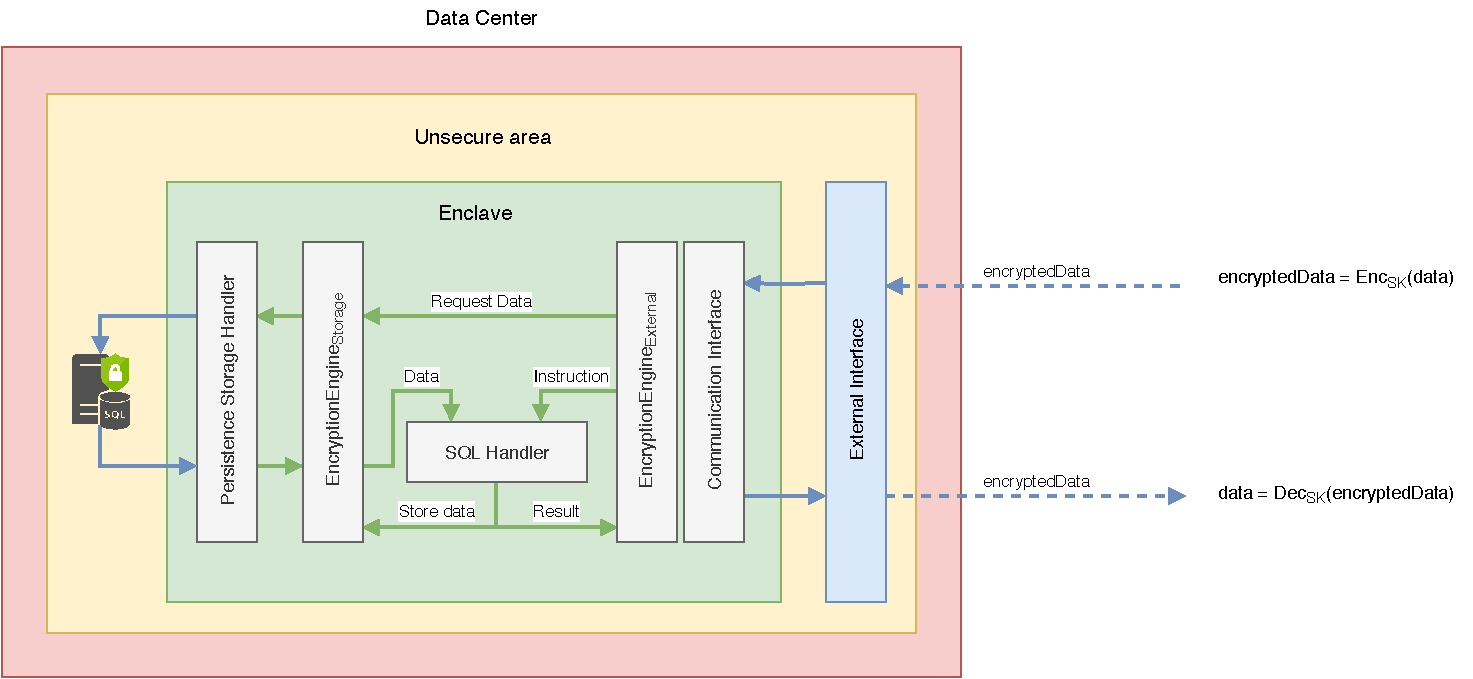
\includegraphics[width=0.8\textwidth]{img/enclave_details/enclave_details.pdf}
 	\caption{Skizzierung des Ziels einer gesicherten Umgebung bei einem \ac{CSP}}
 	\label{img:sgx-idea}
 \end{figure}